\documentclass[11pt]{article}
\usepackage[utf8]{inputenc}
\usepackage{graphicx}
\graphicspath{{figures/}}
\usepackage{times}
\usepackage[margin=0.8in]{geometry}
\usepackage{booktabs}
\usepackage{longtable}
\usepackage{caption}
\usepackage{subcaption}
\usepackage{float}
\usepackage[hidelinks]{hyperref}
\usepackage{url}
\emergencystretch=1.5em
\renewcommand{\thetable}{S\arabic{table}}
\renewcommand{\thefigure}{S\arabic{figure}}

\title{\textbf{Supplementary Information}\\[4pt]
\large Complete Patient-Level Leakage Among Traceable Images in a Widely Used Brain Tumor MRI Benchmark}
\author{Jaiveer Bassi\\Independent Researcher, USA\\\texttt{jaiveerbassi@yahoo.com}}
\date{}

\begin{document}
\maketitle

\section*{Supplementary Methods}
\subsection*{Provenance sensitivity control}
The initial provenance search used ImageNet-pretrained ResNet-18 embedding cosine similarity, histogram-equalized pixel correlation, and intersection-over-union of thresholded brain masks. A byte-identical positive control returned 1.0 under every measure but did not test robustness to transformations introduced by an aggregation pipeline. We therefore constructed transformed-positive controls from known figshare slices. JPEG re-encoding at quality 85--95 and resizing preserved cosine similarity above 0.999, whereas cropping to the brain region reduced median equalized correlation to 0.601 and embedding cosine to 0.963. After crop-normalizing both collections and searching all rotations and reflections, transformed true matches reached median cosine 0.9988 and minimum 0.9884. We used a conservative acceptance threshold of 0.98.

The corrected search matched 4,586 of 5,023 tumor images. Of these, 2,956 matched after a 90-degree rotation and 1,630 after reflection plus a 90-degree rotation; none matched in the identity orientation. Three aggregated images labelled pituitary were labelled meningioma in figshare. The released \texttt{figshare\_patient\_map.json} preserves every accepted score and orientation.

\subsection*{Split checks}
Each patient-disjoint fold was generated from a single cached five-fold assignment. Each recovered patient appears in exactly one test fold. The unmatched tumor images are training-only, and no-tumor near-duplicate clusters are indivisible. Every materialized fold asserts zero group overlap and zero pixel-identical images across the training/test boundary. The random control likewise uses one cached partition rather than five independent draws; every eligible image appears in one test fold, and per-class fold sizes match the patient arm exactly.

\section*{Supplementary Tables}
\begin{table}[H]
\centering
\caption{Composition of the released folders.}
\label{tab:s_dataset}
\begin{tabular}{lrrr}
\toprule
Class & Training & Testing & Total \\
\midrule
Glioma & 1,321 & 300 & 1,621 \\
Meningioma & 1,339 & 306 & 1,645 \\
No tumor & 1,595 & 405 & 2,000 \\
Pituitary & 1,457 & 300 & 1,757 \\
\midrule
Total & 5,712 & 1,311 & 7,023 \\
\bottomrule
\end{tabular}
\end{table}

\begin{table}[H]
\centering
\caption{Crop-normalized, orientation-searched matching against figshare.}
\label{tab:s_provenance}
\begin{tabular}{lr}
\toprule
Quantity & Value \\
\midrule
Transformed control, median cosine & 0.9988 \\
Transformed control, minimum cosine & 0.9884 \\
Acceptance threshold & 0.98 \\
Tumor images matched & 4,586/5,023 (91.3\%) \\
Figshare patients recovered & 233/233 \\
Matched after rotation & 2,956 \\
Matched after reflection and rotation & 1,630 \\
Label disagreements & 3 \\
\bottomrule
\end{tabular}
\end{table}

\begin{table}[H]
\centering
\caption{Exact duplication and within-dataset redundancy by class. ``Unique'' counts distinct decoded pixel contents; clusters additionally collapse embedding cosine similarity $\geq0.99$.}
\label{tab:s_duplicates}
\small
\begin{tabular}{lrrrrr}
\toprule
Class & Test duplicates & \% of test class & Files & Unique & Clusters \\
\midrule
Glioma & 0 & 0.0\% & 1,621 & 1,620 & 1,620 \\
Meningioma & 106 & 34.6\% & 1,645 & 1,531 & 1,522 \\
No tumor & 105 & 25.9\% & 2,000 & 1,706 & 1,113 \\
Pituitary & 5 & 1.7\% & 1,757 & 1,740 & 1,739 \\
\midrule
Total & 216 & 16.5\% & 7,023 & 6,597 & 5,994 \\
\bottomrule
\end{tabular}
\end{table}

\begin{table}[H]
\centering
\caption{Training hyperparameters used for all reported primary runs.}
\label{tab:s_hyperparameters}
\begin{tabular}{ll}
\toprule
Setting & Value \\
\midrule
Architecture & ImageNet-pretrained ResNet-18 \\
Input & $224\times224$, grayscale replicated to RGB \\
Optimizer & Adam \\
Learning rate & $10^{-4}$ \\
Weight decay & 0 (Adam default) \\
Batch size & 32 \\
Maximum epochs & 30 \\
Early stopping patience & 5 epochs \\
Scheduler & ReduceLROnPlateau, factor 0.5, patience 2 \\
Augmentation & Flip; $\pm10^\circ$ rotation; 10\% brightness/contrast \\
Primary seeds & 0, 1, 42 per fold \\
\bottomrule
\end{tabular}
\end{table}

\begin{longtable}{p{0.18\textwidth}p{0.35\textwidth}p{0.37\textwidth}}
\caption{Analyses corrected or superseded during this work. Every result in the submitted manuscript reflects the right-hand column.}
\label{tab:s_corrections}\\
\toprule
Analysis & Earlier problem & Submitted analysis \\
\midrule
\endfirsthead
\toprule
Analysis & Earlier problem & Submitted analysis \\
\midrule
\endhead
Provenance & An identical-file positive control did not test robustness to cropping or orientation changes, producing a false-negative source trace. & Transformed-positive controls motivated crop-normalized, orientation-aware matching, which recovered 4,586 patient identifiers. \\
\addlinespace
Validation split & The initial train/validation division was not grouped by patient, contaminating checkpoint selection, early stopping, and temperature fitting. & All cross-validation runs use group-disjoint validation by recovered patient or no-tumor near-duplicate cluster. \\
\addlinespace
Duplicate errors & A Fisher test treated predictions from ten models on the same images as independent. & Model-level paired and image-level permutation tests preserve correlation; neither reached conventional significance. \\
\addlinespace
Deduplication bound & A bound on inflation was inferred from a $p$-value. & The reported 95\% interval for the accuracy difference is -0.03 to +0.43 points. \\
\addlinespace
Variance claim & Seed variance was compared with an inapplicable binomial floor. & That claim was withdrawn and replaced by per-image agreement and fold-by-seed variance analyses. \\
\addlinespace
Patient estimate & A single partition gave 94.75\% $\pm$ 0.80, where the interval reflected seeds but held the partition fixed. & Five-fold patient-disjoint cross-validation gives 95.19\%; partition variation (2.18 points) exceeds seed variation (0.83 points). \\
\addlinespace
Paired comparison & The initial 1,061-image comparison included 300 no-tumor images without patient identifiers. & Restriction to 761 images with recovered identifiers gives 99.12\% versus 93.60\% and a 7.3-fold error-rate ratio. \\
\addlinespace
Random control & Independently generated folds did not form one matched partition of the evaluation population. & One cached five-fold random partition matches patient-fold class counts and covers the same 6,292 images exactly once per seed. \\
\bottomrule
\end{longtable}

\begin{table}[H]
\centering
\caption{Released-split baseline and ablation results. The main configuration uses ten seeds; the other ablation cells use five.}
\label{tab:s_ablation}
\begin{tabular}{lrrr}
\toprule
Augmentation & Backbone & Accuracy & SD \\
\midrule
On & Fully fine-tuned & 99.22\% & 0.16 pt \\
Off & Fully fine-tuned & 98.66\% & 0.47 pt \\
On & Frozen & 83.57\% & 0.42 pt \\
Off & Frozen & 84.99\% & 0.31 pt \\
\bottomrule
\end{tabular}
\end{table}

\begin{table}[H]
\centering
\caption{Complete run inventory. Prediction files and per-run histories are available under \texttt{runs/}; aggregate metrics are stored in each tagged directory.}
\label{tab:s_runs}
\small
\begin{tabular}{lll r}
\toprule
Tag & Configuration & Evaluation & $n$ \\
\midrule
\texttt{leaky} & Augmented, full fine-tuning & Released holdout & 10 \\
\texttt{dedup} & Augmented, full fine-tuning & Deduplicated holdout & 10 \\
\texttt{cv\_fold0--4} & Augmented, grouped validation & Patient-disjoint CV & 15 \\
\texttt{rand\_fold0--4} & Augmented, grouped validation & Random-fold control & 15 \\
\texttt{patient} & Augmented, ungrouped validation & Retired single partition & 5 \\
\texttt{abl\_noaug\_full} & No augmentation, full fine-tuning & Released holdout & 5 \\
\texttt{abl\_aug\_frozen} & Augmented, frozen backbone & Released holdout & 5 \\
\texttt{abl\_noaug\_frozen} & No augmentation, frozen backbone & Released holdout & 5 \\
\midrule
\multicolumn{3}{l}{Total} & 70 \\
\bottomrule
\end{tabular}
\end{table}

\section*{Supplementary Figures}
\begin{figure}[H]
\centering
\begin{subfigure}[t]{0.48\textwidth}
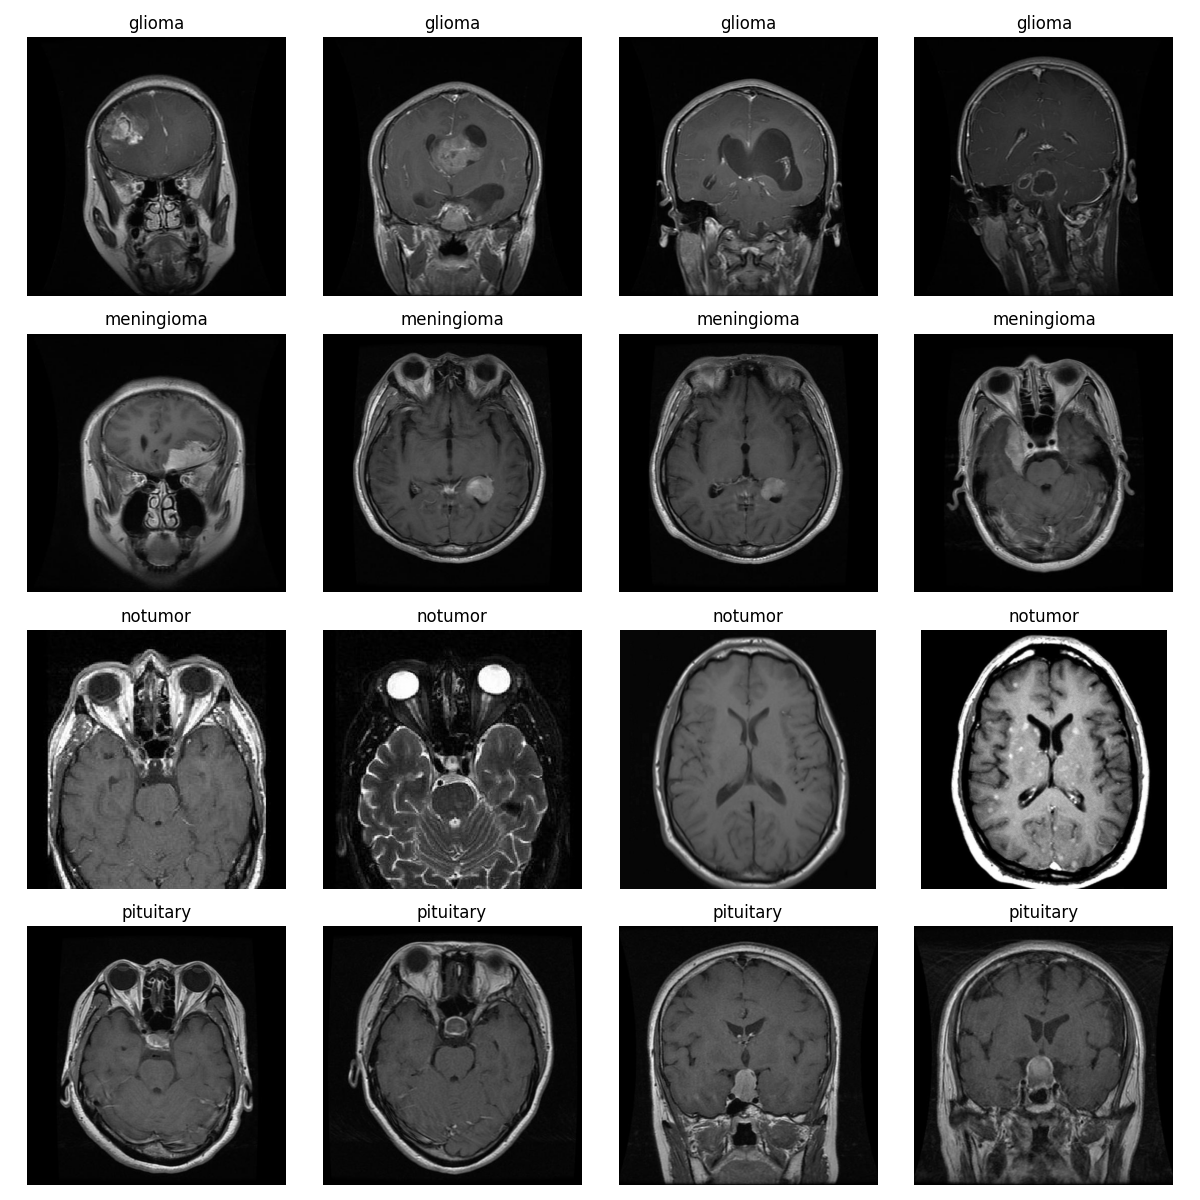
\includegraphics[width=\linewidth]{Figure_1.png}
\caption{One example from each class.}
\end{subfigure}\hfill
\begin{subfigure}[t]{0.48\textwidth}
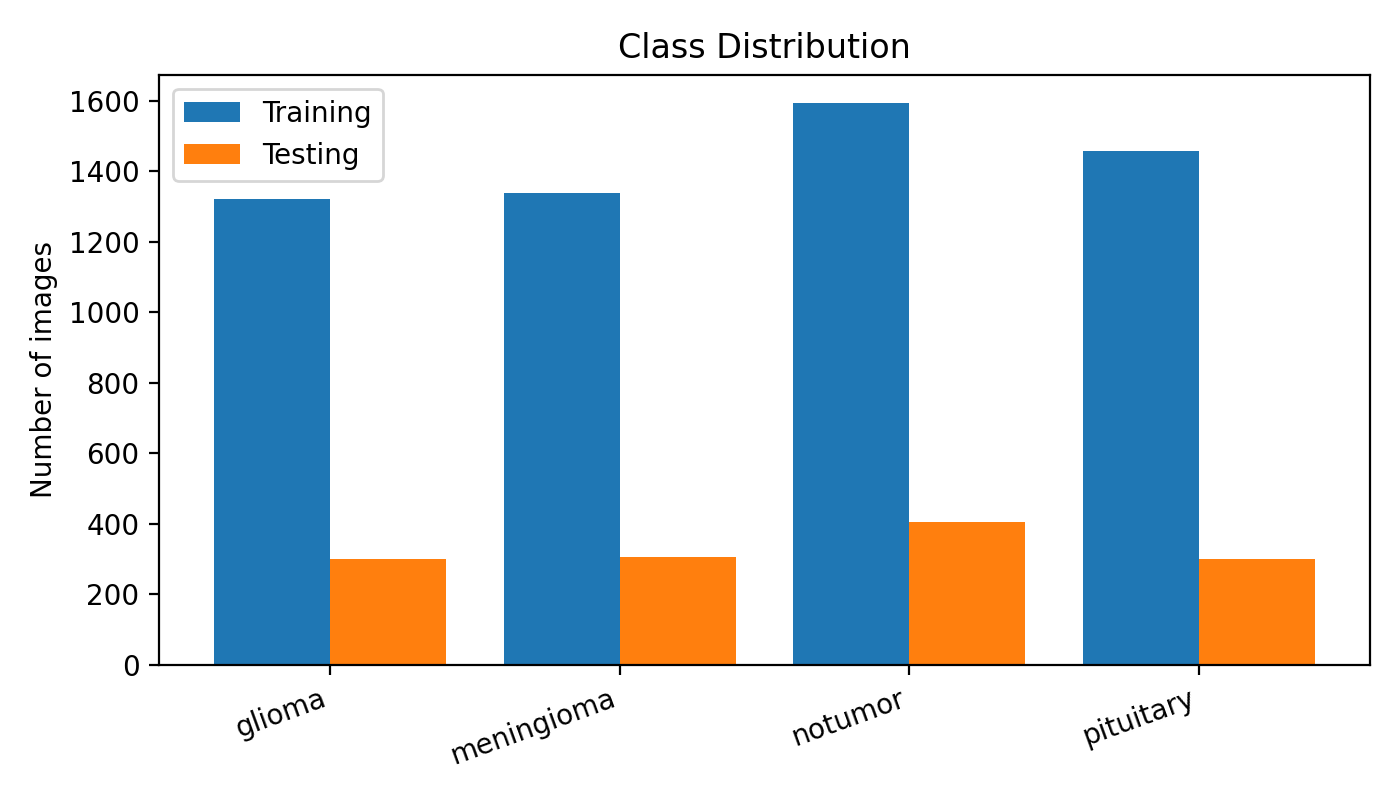
\includegraphics[width=\linewidth]{class_distribution.png}
\caption{Released folder counts by class.}
\end{subfigure}
\caption{Dataset examples and class distribution.}
\label{fig:s_dataset}
\end{figure}

\begin{figure}[H]
\centering
\begin{subfigure}[t]{0.48\textwidth}
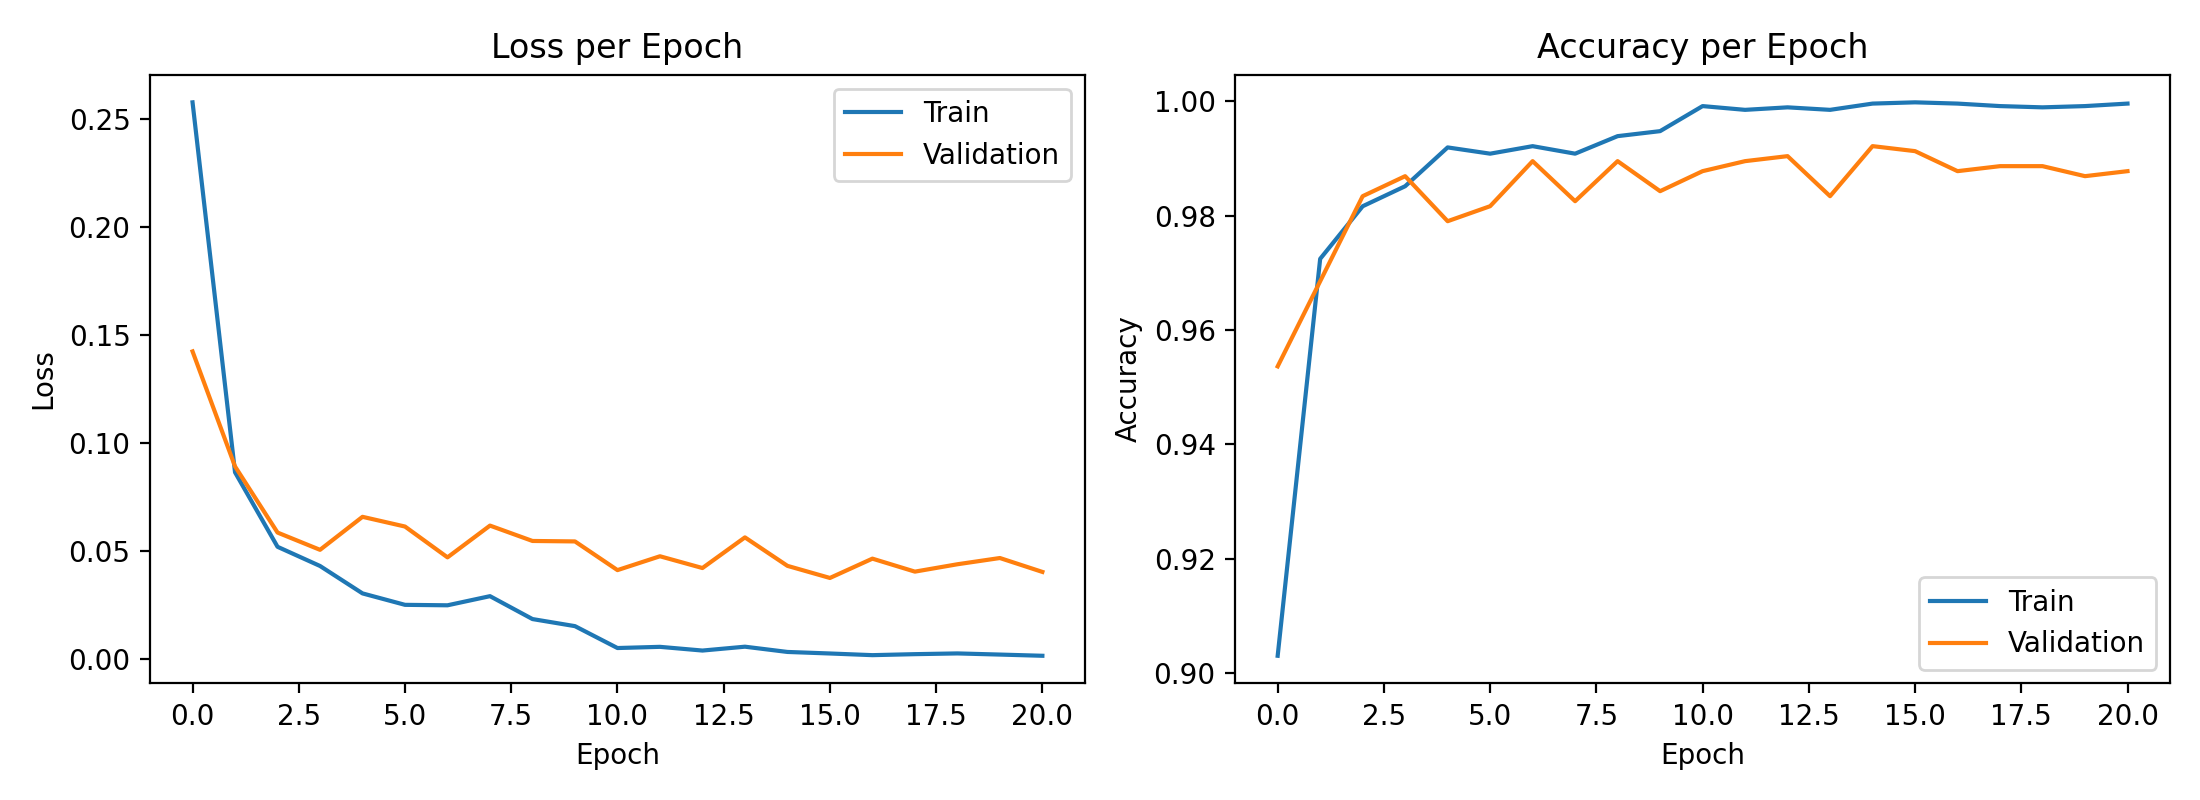
\includegraphics[width=\linewidth]{training_curves.png}
\caption{Training and validation loss and accuracy.}
\end{subfigure}\hfill
\begin{subfigure}[t]{0.48\textwidth}
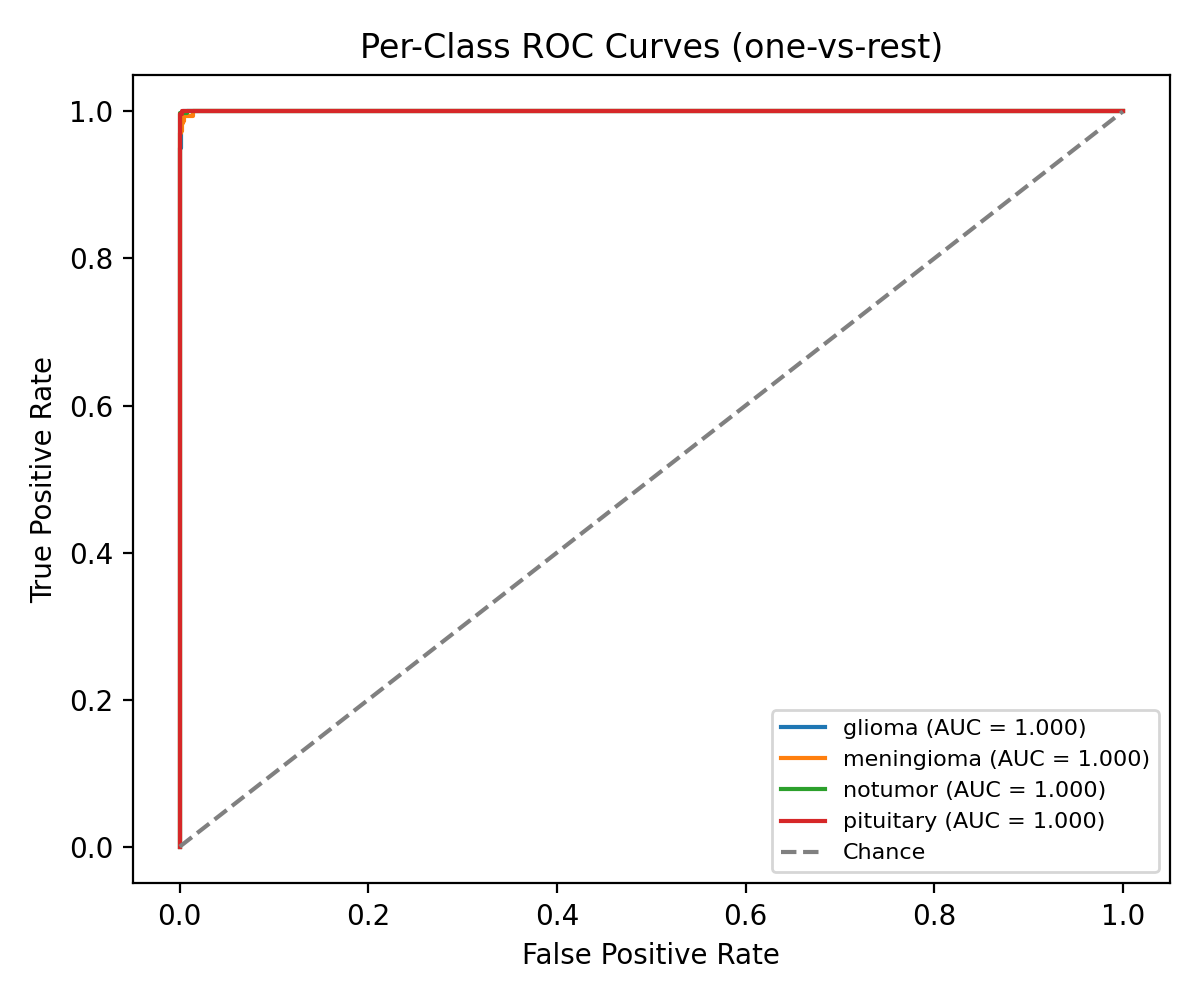
\includegraphics[width=\linewidth]{roc_curves.png}
\caption{Released-split one-versus-rest ROC curves.}
\end{subfigure}
\caption{Released-split training dynamics and ranking performance. These results are measured under patient leakage.}
\label{fig:s_training}
\end{figure}

\begin{figure}[H]
\centering
\begin{subfigure}[t]{0.45\textwidth}
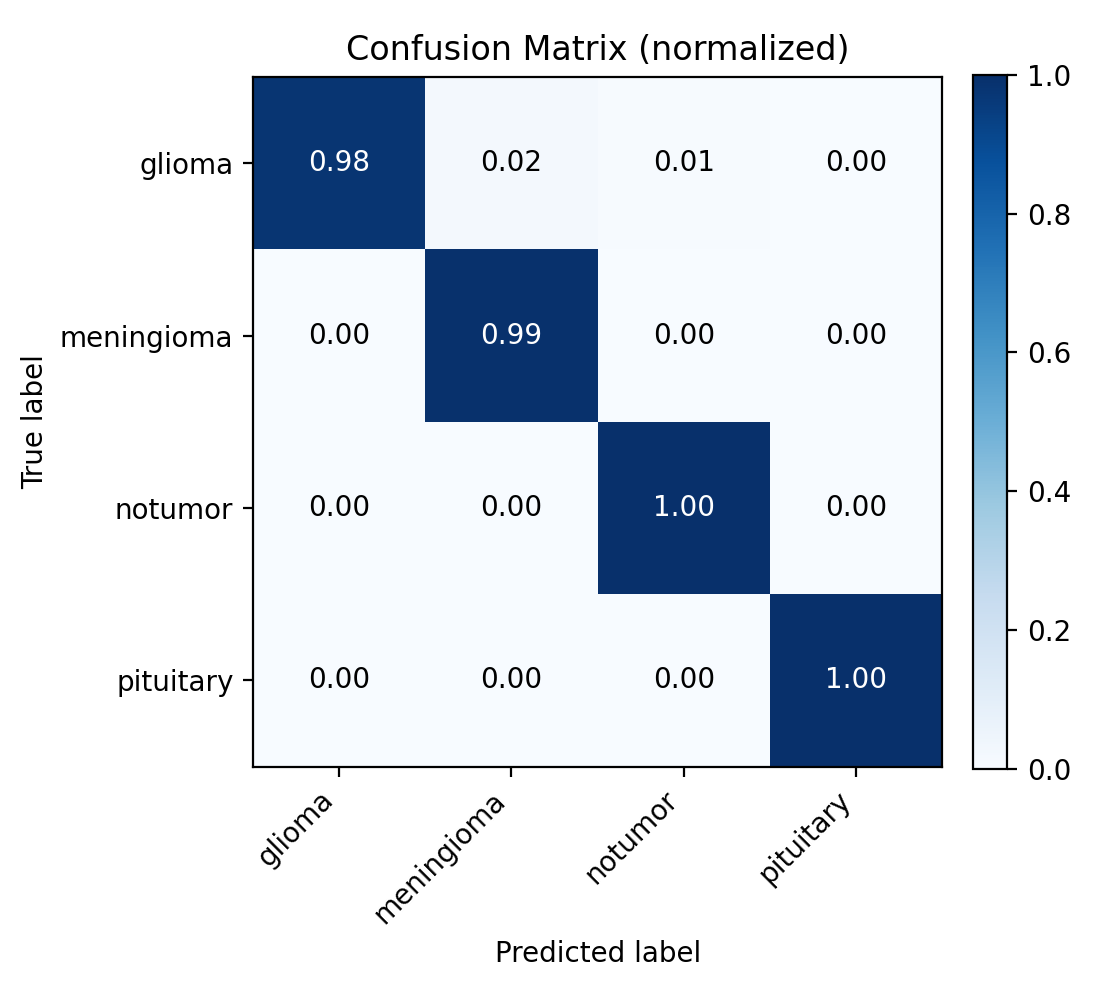
\includegraphics[width=\linewidth]{confusion_matrix.png}
\caption{Normalized confusion matrix.}
\end{subfigure}\hfill
\begin{subfigure}[t]{0.52\textwidth}
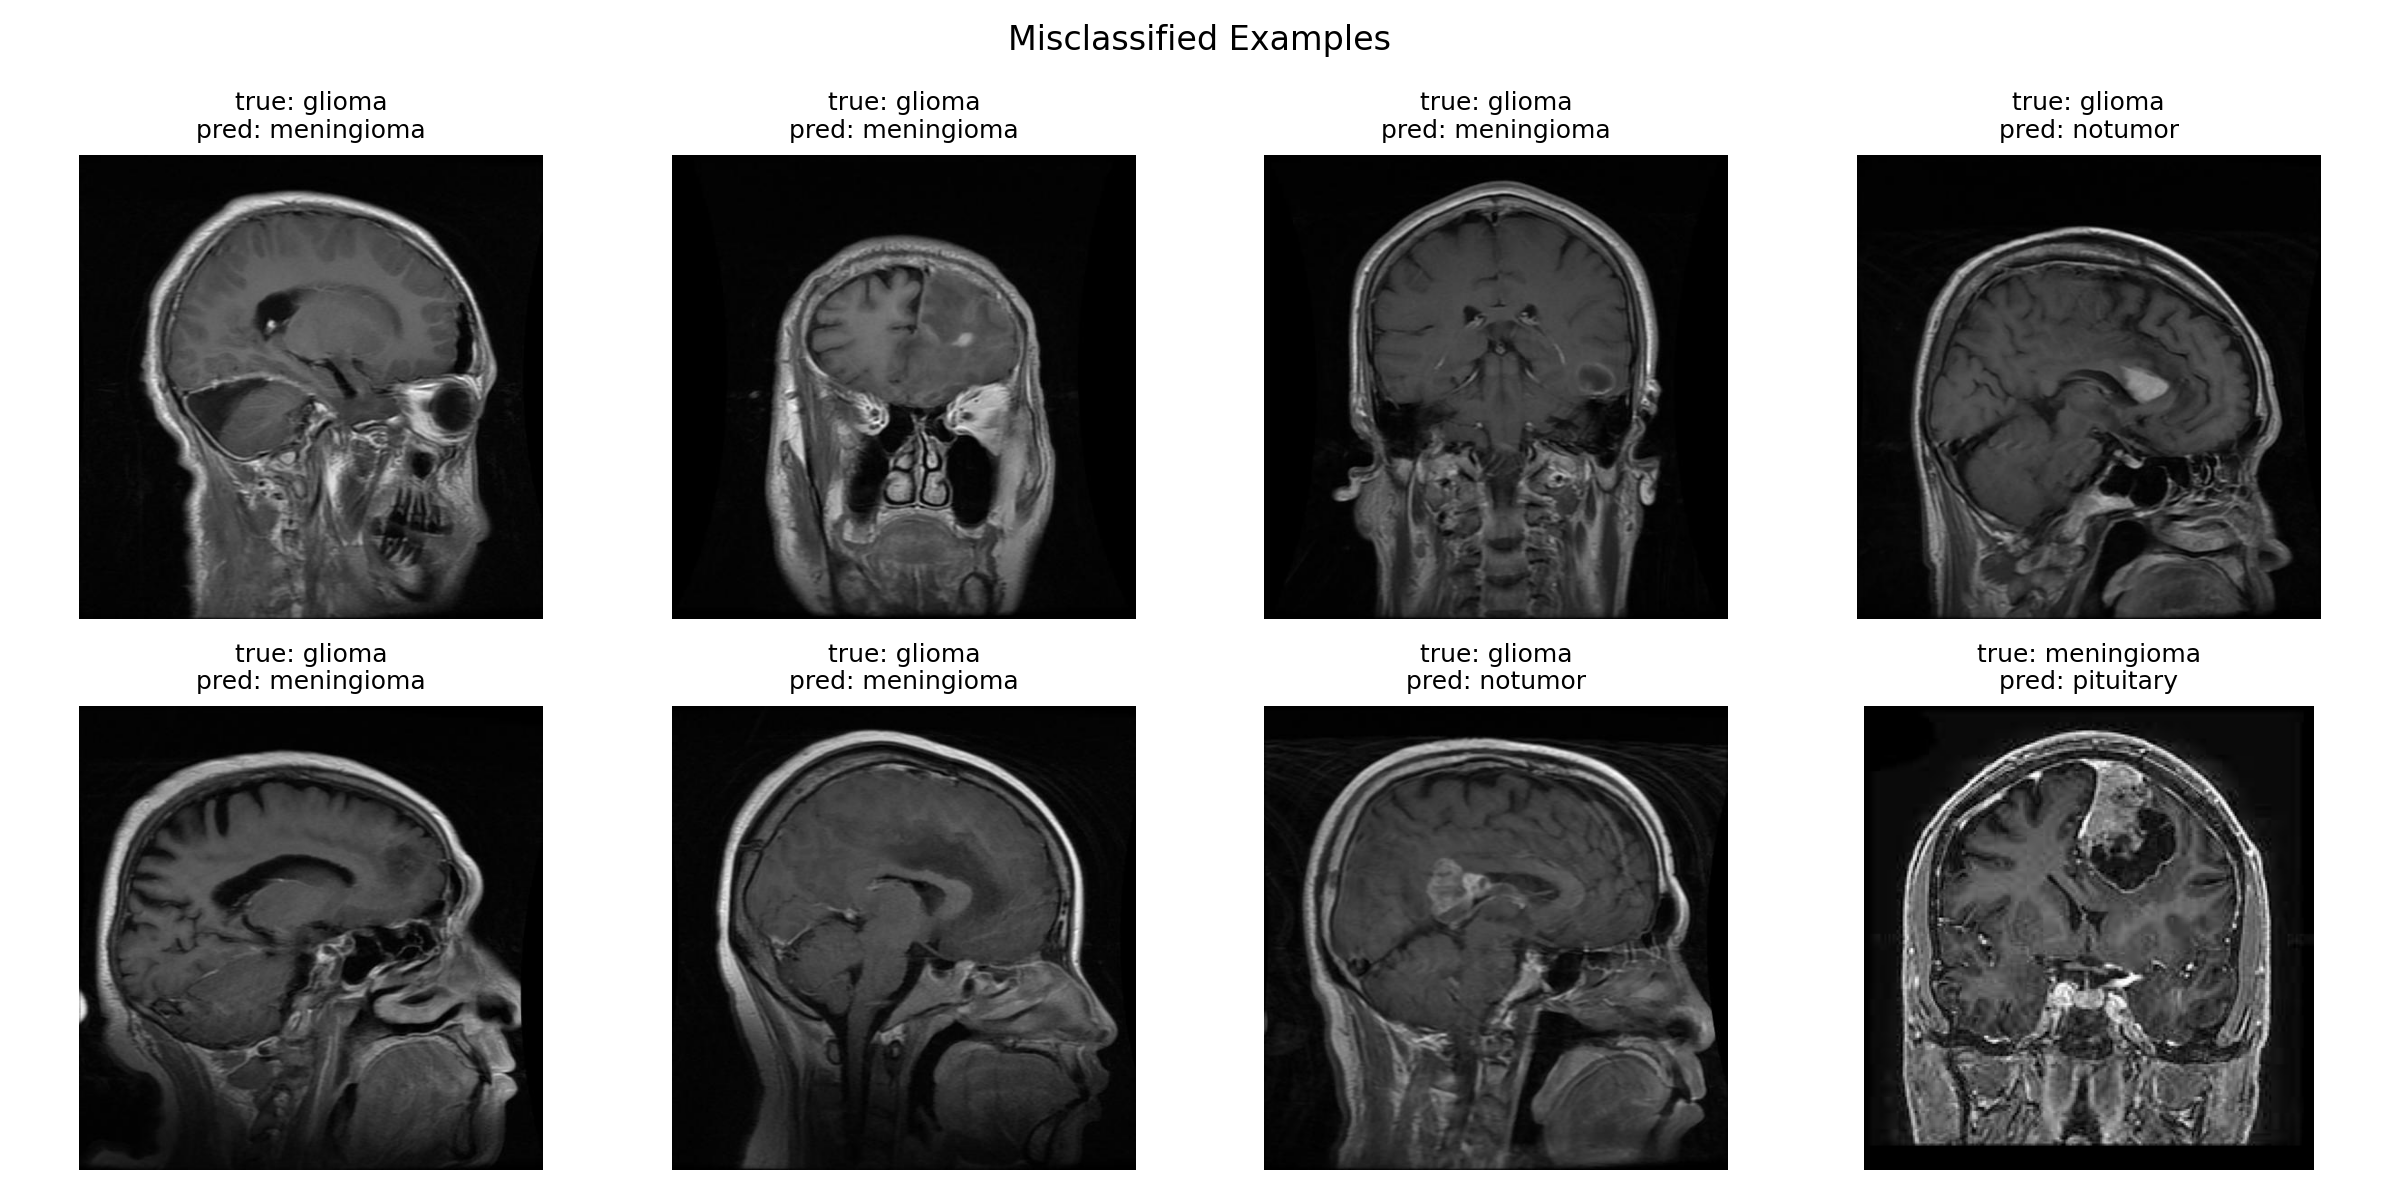
\includegraphics[width=\linewidth]{misclassified_examples.png}
\caption{Released-split errors.}
\end{subfigure}
\par\medskip
\caption{Released-split error analysis, provided for reproducibility rather than as evidence of generalization.}
\label{fig:s_errors}
\end{figure}

\end{document}
